\chapter{质点动力学(一)}
前面说过,动力学研究物体运动状态的变化和物体与外界相互作用的关系。在经典力学中外界对物体的作用指的就是力的作用,质心运动状态通常指的是质点的位置矢量$\vec{r}$和速度矢量$\vec{v}$,运动状态的变化用$\dot{\vec{r}}$和$\dot{\vec{v}}$表示,所谓动力学规律就是指$\dot \vec{r}$,$\dot \vec{v}$与作用力$\vec{F}$的关系,这是关于$\dot \vec{r}$,$\dot \vec{v}$的一个方程组(一阶微分方程组),由于$\dot{\vec{r}}=\vec{v}$,因此也可以表示为$\vec{r}$的二阶微分方程。通常把它称作运动微分方程。这一张我们要讨论建立运动方程的一般步骤,并在一些简单情况下求解相应的运动微分方程。
\[\text{\simhei{动力学:}}\text{物体运动状态变化与物体和外界相互作用的关系}\]
\[\begin{CD}
\vec{r_1},\vec{v_1} @>\vec{F}>> \vec{r_2},\vec{v_2}
\end{CD}\]
\begin{center}
$\dot{\vec{r}},\dot{\vec{v}}$与$\vec{F}$是关于$\dot{\vec{r}},\dot{\vec{v}}$的一个微分方程(一阶微分方程组)(因为$\vec{v}=\dot{\vec{r}},\dot{\vec{v}}=\frac{d^2\vec{r}}{dt^2}$)
\end{center}
\section{牛顿第一定律、惯性参照系}
\subsection{牛顿第一定律}每个物体将继续保持静止或沿一直线匀速运动的状态,除非有力加于其上,迫使它改变这种状态。
\subsubsection{关于“力”的概念}定性地说,是迫使物体改变静止或匀速直线运动状态的一种作用。使$\vec{a}=0\ \to\ \vec{a}\ne 0$。力这一定义大大拓宽了力的概念,使力的范畴从原来的仅限弹性力、肌肉力、压力拓展到包括引力,电磁力等(从接触力道非接触力(场力))。
\subsubsection{关于“惯性”的概念}物体在不受力的情况下保持其静止或匀速直线运动状态的属性。惯性不仅在不受力的情况下有所表现,在受力时也表现惯性——惯性质量——惯性的度量。
第一定律又称惯性定律(指物体具有惯性)。

\section{惯性参照系}
牛顿第一定律成立的参照系叫做惯性参照系;惯性参照系不受其它物体作用。

由前面运动学部分的分析,可知惯性参照系不可解只有一个,而是所有彼此相对静止或做匀速直线运动的参照系具有等价性:一个是惯性系,其他也是惯性系;一个不是惯性系,其他也不是惯性系。

有牛顿第一定律也可知,作为惯性系的参照物必定不受力(不受其他物体的作用)。

实际上并不存在严格意义下的惯性系,只有远离其他物体的作用的孤立物体都可近似看作惯性参照系。

请看下面一组数据:

地面相对地心参照系,自转加速度为$3.4\times 10^{-2}m/s^2$

地心参照系相对太阳参照系,公转加速度$5.9\times 10^{-3}m/s^2$

太阳对银河系中心旋转使其对银心有$10^{-10}m/s^2$的加速度

更好一些的参照系,$FK_4$系,是以选定的$1535$颗恒星的平均静止位形作为基准的参照系

另以射电源为基准的参照系,以及以微观背景辐射为基准的参照系。

有关惯性系问题的解决是在爱因斯坦建立广义相对论以后。
\section{牛顿第二定律(质量和力的量度)}
\[\vec{F}=m\vec{a}\text{(惯性参考系)}\]
\begin{align}
\text{\simhei{质量的度量}:}&
\text{在相等的力作用下,两个物体的加速度分别为}\vec{a_1},\vec{a_2}\text{,则}\frac{m_1}{m_2}=\frac{\vec{a_1}}{\vec{a_2}}\text{,即}m_2=m_1\frac{\vec{a_1}}{\vec{a_2}} \notag \\
\text{\simhei{力的度量}:}&
\text{以牛顿第二定律为基础,规定单位质量}1kg\text{的质点获得单位加速度}1m/s^2\text{的力为一个单位力,} \notag \\
&\text{称为}1\text{牛顿(}1N\text{),即}1N=1kg\times1m/s^2 \Rightarrow 1N=1kg\cdot m/s^2 \notag
\end{align}
\section{常见的力}
\subsection{万有引力}
\[\vec{F_{12}}=-\frac{Gm_1m_2}{r_{12}^2}\hat{r_{12}}\]
\begin{center}
$\hat{r_{12}}$表示此力是$\vec{r_{12}}$方向上的力\\$G=6.67\times 10^{-11}Nm^2/kg^2=6.67\times10^{-11}m^3/s^2kg$
\end{center}
\subsubsection{重力}地面表面附近地球对物体的万有引力
\[F=\frac{GM_em}{R_\omega^2}=mg\]\[g=\frac{GM_e}{R_e^2}\text{(重力加速度)}\]
\subsection{弹性力}
物体因形变而产生的恢复力称为弹力
\subsubsection{胡克定律}
大多数物体当\underline{形变不大}时,其恢复力与形变成正比,这是一个经验规律。
\[F=-kx\quad\text{($k$为弹性系数)}\]
\subsection{摩擦力}
当两个物体的接触面有相对滑动或有相对运动趋势时,会产生一种阻碍相对滑动或相对滑动趋势的力叫做摩擦力。固体与固体之间的摩擦力叫做干摩擦力,液体不同流层之间由于相对滑动产生的阻力叫做湿摩擦力或粘滞阻力
\subsubsection{摩擦定律}$f_N=\mu_k N$
\subsubsection{粘滞定律}$F=\eta\varDelta S \frac{dv}{dz}$,其中$\varDelta$为面积,$\frac{dv}{dz}$为速度的横向变化率或横向梯度,$\eta$为粘度系数(粘度),$\eta$取决于材料(流体)本身。

固体与流体之间发生相对运动时,当速度不大时,$\vec{F}=-\alpha\vec{v}$
\subsection{洛伦兹力}
带电粒子在电磁场中受的力:$\vec{F}=q(\vec{E}+\vec{v}\times\vec{B})$
\section{牛顿定律的运用、运动微分方程的建立}
\subsection{质点动力学的基本问题}
在一定力的作用下(包含给定初始条件)求解物体的运动以及根据物体求其所受的力。
\subsubsection{求解步骤}
\begin{enumerate}
\item 明确考察对象
\item 选定参考系与坐标系
\item 根据力的定律的运动定律,写出运动方程或运动方程组,由于运动的矢量性,在选定坐标系后将矢量微分方程改写为标量微分方程
\item 用代数的,几何的和分析的方法来求解运动方程
\item 分析讨论
\end{enumerate}
\subsection{例题分析}
\subsubsection{一维谐振子}
作用力:$\vec{F}=-kx$,即$m\frac{d^2x}{dt^2}=-kx$
\begin{figure} [ht]
\centering
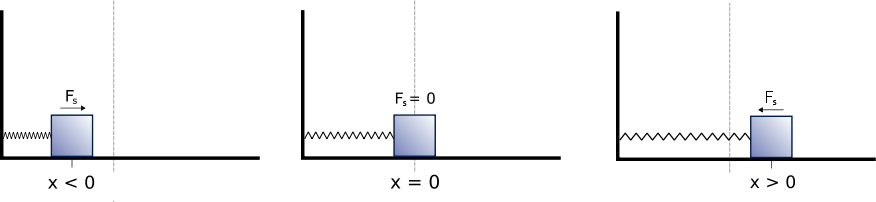
\includegraphics[scale=.5]{308px-Harmonic_oscillator.svg.png}
\caption{\simsun 一维谐振子}
\label{308px-Harmonic_oscillator.svg.png}
\end{figure}

令$\omega^2=\frac{k}{m}$(注意$\omega^2$的量纲:$[w^2]=\frac{\frac{kg\cdot m/s^2}{m}}{kg}=\frac{1}{s^2}$)得一维谐振子方程:
\[\frac{d^2x}{dt}+\omega^2x=0 \tag{*}\]

上式为二阶常系数齐次线性微分方程,这类方程的一般形式是
\[\frac{d^2x}{dt^2}+b\frac{dx}{dt}+cx=0\]
对于这类方程一般的解法如下:设$x(t)=e^{at}$,带入原方程得
\[(a^2+ba+c)e^{at}=0\]
上式称为原方程的特征方程,解得$a_1,a_2$,若$a_1\ne a_2$,则$e^{a_1t}$和$e^{a_2t}$就是原微分方程的两个彼此独立的解,方程的通解为它们的线性组合:
\[x(t)=c_1e^{a_1t}+c_2e^{a_2t}\]

考虑(*)式,它的特征方程是:
\[\lambda^2+\omega^2=0 \ \Rightarrow \  \lambda_1=\omega i\,, \lambda_2=\omega \]
\[ \therefore x_1(t)=e^{\omega i t},\,x_2(t)=e^{-\omega i t}\]
作$x_1(t),x_2(t)$的线性组合(由欧拉公式):
\[x_1'(t)=\frac{x_1+x_2}{2}=\cos\omega t\,,x_2'(t)=\frac{x_1-x_2}{2}=\sin\omega t\]
所以(*)的解为:
\[x(t)=c_1'x_1'+c_2'x_2'=A\cos(\omega t+\varphi)\]
其中$A$叫做\underline{振幅},$\varphi$叫做\underline{初相}。
\subsubsection{受阻下落}
设在空气中自由下落的物体受空气的阻力$\vec{F}$满足关系$\vec{F}=-\alpha\vec{v}$,则:
\[m\vec{a}=mg-\alpha\vec{v}\ \Rightarrow \ m\frac{d^2z}{dt^2}=mg-\alpha\frac{dz}{dt}\]
整理成标准形式
\[\frac{d^2z}{dt^2}+\frac{\alpha}{m}\frac{dz}{dt}=g\tag{**}\]
上式为二阶常数非齐次线性微分方程,它诱导的齐次微分方程如下:
\[\frac{d^2z}{dt^2}+\frac{\alpha}{m}\frac{dz}{dt}=0\]
设$z_1(t),z_2(t)$是上述齐次方程的两个独立的解,再设$z_s(t)$是方程(**)的一个特解,则方程(**)的一般解为
\[z(t)=z_s(t)+c_1z_1(t)+c_2z_2(t)\]
易解得$z_1=e^{-\frac{\alpha}{m}m},z_2=1$,再用以下方法求$z_s(t)$:设$z_s(t)=at$,代入(**)式:
\[\frac{\alpha}{m}a=g \ \Rightarrow\ a=\frac{mg}{\alpha}\]
\[\therefore z_s(t)=\frac{mg}{\alpha}t\]
综上所述:
\begin{align}
z&=c_1e^{-\frac{\alpha}{m}t}+c_2+\frac{mg}{\alpha}t \notag \\
&=c_1e^{-\frac{t}{\tau}}+c_2+v_ct\notag
\end{align}
由初始条件$t=0$时$z=0$得:
\[c_1+c_2=0\]
再由初始条件$t=0$时$\frac{dz}{dt}=0$,得:
\[-\frac{c_1}{\tau}+v_c=0\]
因此
\[c_1=v_0\tau,\,c_2=-v_c\tau\]
最终解得
\[z=v_c\tau\left(e^{-\frac{t}{\tau}}-1\right)+v_ct\]
\subsubsection{在太阳引力作用下讨论行星运动}
\begin{align}
\vec{F}&=-\frac{GMm}{r^2}\hat{r}=m\frac{d^2\vec{r}}{dt} \notag \\
\hat{r} &= \frac{x\vec{i}+y\vec{j}+z\vec{k}}{\sqrt{x^2+y^2+z^2}} \notag
\end{align}
可以证明,在有心力作用下质点做平面运动(见后)由于作用力为有心力,在平面极坐标系下考虑这个问题比较方便,此时外力只在$\vec{e_r}$方向有作用:
\[\begin{cases}
m(\ddot{r}-r\dot{\varphi}^2)=-\frac{GMm}{r^2}\\
m(2\dot{r}\dot{\varphi}+r\ddot{\varphi})=0
\end{cases}
\]
此为二阶非线性微分方程组,求解此方程组比较复杂,需利用方程组的两个初积分(或两个运动积分)
\[\begin{cases}
mr^2\dot{\varphi}=G_0,\,\text{角动量守恒}\\
\frac{1}{2}m(\dot{r}^2+r^2\dot{\varphi}^2)+V(r)=E,\text{机械能守恒}
\end{cases}
\]
得
\[
\frac{1}{2}m\dot{r}^2+V_{eff}(r)=E\,\text{其中第二项为有效势能}
\]
\[V_\text{eff}=\frac{G_0^2}{2mr^2}+V(r)\]
得
\[\dot{r}=\pm \sqrt{\frac{2}{m}[E-V_{eff}(r)]}\]
分离变数,得
\[dt=\frac{\pm dv}{\sqrt{\frac{2}{m}[E-V_{eff}(r)]}}\]
\[t=\int_{r_0}^r \frac{\pm dv}{\sqrt{\frac{2}{m}[E-V_{eff}(r)]}}\]
积分求得$r(t)$,再代入角动量守恒方程得
\[d\varphi = \frac{G_0 dt}{mr^2(t)}\]
求得
\[\varphi(t)=G_0\int_0^t \frac{dt}{mr^2(t)}+\varphi_0\]
在讨论太阳引力作用下行星的运动,其运动情况稍微简单一些。由运动方程组可推导出轨道微分方程,并求出其相应的轨道。
\subsection{初积分}
如果方程$G(x,y,z,\dot x,\dot y,\dot z,t)=c$对时间的一次微商是牛顿运动方程,就称上式为牛顿运动方程的初积分,或第一积分,从数学上看初积分使牛顿运动方程从二阶方程降为一阶方程,从物理上看,它表示某个力学量是运动守恒量。
\begin{align}
G_1&=r^2\dot\varphi=c \notag \\
\frac{G_2}{dt}&=2r\dot r\dot\varphi+r^2\ddot \varphi = r(2\dot r\dot\varphi+r\ddot\varphi)=0\notag \\
G_2&=\frac{1}{2}m(\dot r^2+r^2\dot{\varphi^2})-\frac{GMm}{r}=c_2 \notag \\
\frac{G_2}{dt}&=\frac{1}{2}m(2\dot r\ddot r+2 r \dot r \dot\varphi^2+2 r^2\dot\varphi\ddot\varphi)+\frac{GMm}{r^2}\dot{r}=0 \notag \\
\frac{G_2}{dt}&=\frac{1}{2}m(2\dot r\ddot r+2r \dot r \dot\varphi^2-4r\dot\varphi\dot r\dot\varphi)+\frac{GMm}{r^2}\dot{r}=0 \notag
\end{align}
\begin{align}
\dot r\left[ m(\ddot r-r\dot\varphi^2)+\frac{GMm}{r^2}\right]&=0 \notag \\
\frac{1}{2}m\dot r^2+\frac{mG^2}{2mr^2}-\frac{GMm}{r}&=c_2 \notag
\end{align}
\[ \Rightarrow r=\pm \sqrt{\frac{2}{m}\left[ c_2-\frac{c_1^2}{2r^2}+\frac{GMm}{r}\right] }\]
\section{质点在非惯性系中的运动、惯性力}
\subsection{非惯性系}
常常需要去非惯性参照系中讨论物体的运动,依照参照系变换时运动学量的变换关系,特别是加速度的变换关系,研究由惯性系中质量的运动方程推出非惯性参照系中质点的运动方程。

已知在惯性参照系中质点的运动服从牛顿第二定律
\[m\frac{d^2 \vec{r}}{dt^2}=\vec{F}\]
若已知非惯性参照系与惯性参照系的加速度的变换关系,例如:
\subsubsection{$S'$相对$S$作任意方式平动}由参照系变换公式和牛顿第二定律:
\[m(\vec{a'}+\vec{\omega})=\vec{F}\  \Rightarrow \ m\vec{a'}=\vec{F}-m\vec{\omega}=\vec{F}+\vec{F_i}\]

其中$\vec{F_i}$称作平移惯性力。
\subsubsection{$S'$相对$S$作匀角速度转动}由参照系变换公式和牛顿第二定律:
\[m(\vec{a'}+\vec{a_c}+\vec{a_{col}})=\vec{F}\]
\begin{align}
 \Rightarrow m\vec{a'}&=\vec{F}-m\vec{\omega}\times(\omega\times\vec{r'})-m2\vec{\omega}\times\vec{v'}\notag \\
 &=\vec{F}+\vec{F_c}+\vec{F_{col}}\notag \\
 &=\vec{F_{eff}} \notag
 \end{align}

其中 $\vec{F_c}$称作惯性离心力,$\vec{F_{col}}$称作科里奥利力,$\vec{F_{eff}}$称作表观力。可见在非惯性系下:\[ m\vec{a}=\vec{F_{eff}}\]

也即是在非惯性系中,质点的运动仍满足牛顿第二定律,只不过必须认为作用在质点的力除了真实的作用力$\vec{F}$外,还有虚拟的惯性力$\vec{F_i}$作用,即表观力的作用下的运动。

应该指出惯性力与真实力不同,无法指出惯性力的施力对象,也无法指出其反作用力,因此对惯性力无法涉及牛顿第三定律。但是在非惯性系中,在讨论质点运动时,它与真实力有着相同的效果。
\subsection{应用惯性力分析物理现象}
\subsubsection{在人造卫星或宇宙飞船绕地球运动时在舱内所看到的失重现象}
在人造地球卫星或宇宙飞船绕地球飞行时,卫星或飞船相对于地球有一心向加速度,在近地附近近似等于重力加速度。卫星或飞船参照系相对于地球的加速度也是这个加速度。因此在卫星参照系中物体所受的表观力(表观重力)为零,失重就是指的表观重力等于零(消失了)。
\begin{description}

\item[在地面上看]卫星以加速度$\vec{g}$绕地球转动:
\[m\vec{a}=m\vec{g}\]
\item[在卫星里看]在卫星里看,表观力为$0$,因此称为失重(但不是不受力):
\[m\vec{a'}=m\vec{g}+\vec{F_i}=m\vec{g}-m\vec{\omega}=0\]
\end{description}
\subsubsection{重力与纬度的关系}
\[\vec{F_i}=-m\vec{\omega}\times(\vec{\omega}\times\vec{r})\]
\[\vec{F_{eff}}=\vec{G}+\vec{F_i}=\vec{w}\]
\[\vec{F_i}:\text{惯性离心力}\]
\[\vec{G}:\text{地球引力(重力)}\]
\[\vec{w}:\text{表观重力}\]
$G=mg_0,F_i=m\omega^2 R cos\lambda,\omega$(地球自旋角速度)$=\frac{2\pi}{86400}\approx 7.29\times 10^{-5}/s,R$(地球半径)$\approx 6.4\times 10^6 m,\lambda:$纬度角
\begin{align}
w&=\sqrt{G^2+F_i^2-2GF_i \cos \lambda} \notag\\
&=G(1-\frac{F_i}{G}\cos\lambda\notag \\
&=mg_0(1-\frac{1}{289}\cos^2\lambda)\notag
\end{align}
\[\frac{\omega^2 R^3}{GM}=\frac{1}{289}\]
\[K=6.37\times 10^6m\, M=5.98\times 10^24kg\]
\[G=6.6726\times 10^{-11}m^3/kg\cdot s^2\]
令$w=mg$,
\[g=g_0(1-\frac{1}{289}\cos^2\lambda)\]
上式反映了重力$w$(因而重力加速度$g$)随纬度的变化。
\subsubsection{在地球上观测的科里奥利力}
科里奥利力:$\vec{F_{col}}=-2m\vec{\omega}\times\vec{v}=2m\vec{v}\times\vec{\omega}$

在北半球:河流对右岸冲击加剧;自由落体偏东;傅科摆。

有三个特征:
\begin{enumerate}
\item 与相对速度成正比,故只有当物体相对参照系运动时才可能出现;
\item 与转动参照系的加速度的一次方成正比,故当角速度较小时,科里奥利力比惯性离心力更重要
\item 力的方向总是与相对速度垂直,故不会改变相对速度大小,但却一定时时刻刻去改变运动的方向
\end{enumerate}

科里奥利力在地球上的表观:北半球:河流对右岸冲击加剧;火车对右轨的偏压较大;落体偏东;傅科摆。